% chap1.tex
\part{서론}
\label{part:introduction}

% ---------------------------------------------------------------------------- %
%                                  NEW SECTION                                 %
% ---------------------------------------------------------------------------- %

\chapter{개발 배경 및 원리}

\section{동적 시뮬레이션 기반 그린리모델링 의사결정 지원도구}
(필요성에 대한 서술 필요)\cite{van2018epb}.

@TODO 
NDC 2030 그린리모델링 국내에서는 평가도구가 부실한 실정임. 기축건물을 위한 ECO2-OD가 있긴 하지만, 그린리모델링은 기술간의 교호작용을 고려할 수 있는 동적으로 평가하는 것이 맞음 [형곤 AIK citation]. 하지만 EnergyPlus는 사용자가 입력하기에 너무 많은 입력 변수를 요구, 조건 1) 2) 3)을 만족하는 시뮬레이터가 요구됨.

% ---------------------------------------------------------------------------- %
%                                  NEW SECTION                                 %
% ---------------------------------------------------------------------------- %

\section{\simulator의 접근 및 철학}

\subsection{원칙}
ECO2 입력 수준 만큼의 노력으로 high-fidelity 동적 시뮬레이션 가능하게 하는 걸 목적으로 하여, 아래 원칙들을 지키며 만들었음.

\begin{itemize}
  \item 기존에 국내에서 쓰이던 건물 에너지 평가 도구의 입력 수준과 유사
  \item EnergyPlus 엔진을 사용하여 건물의 동적 거동 상세하게 모사
  \item 기축건물에서 사용자가 얻기 어렵지만, 동적 시뮬레이터에서 요구하는 것들 가정 (normative dynamic)
  \item ASHRAE F., 건축물에너지효율등급인증규정 등 국내외 기준 참고하여 표준적인 시뮬레이션이 가능하도록 함.
\end{itemize}

\subsection{다른 도구들과의 관계}
\subsubsection{EnergyPlus, DesignBuilder}
\simulator\는 EnergyPlus의 wrapper로 볼 수 있음. EnergyPlus는 엔진의 역할, DesignBuilder가 그걸 포장하는 툴인데, \simulator~도 비슷한 관점에서 만들어진 것임. 단, DesignBuilder는 높은 자유도를 거의 그대로 보장하고 사용 가능한 dataset도 그냥 열린 반면에, 우리 \simulator\는 국내 실정과 기축건물의 그린리모델링이라는 상황에 적합하게 커스터마이징하여, 쉽게 사용 가능.

\subsubsection{ClimateStudio, Honeybee}
둘 다 EnergyPlus의 wrapper인데, Raw-level에서의 수정도구인 DesignBuilder보다는 좀 더 graphical code 개념도 쓰고 해서 좀 더 구조적인 모델링이 가능하도록 만든 것임. \simulator~의 자료구조와 python 코드상의 구조는 두 프로그램을 참고하여 만들었음.

\subsubsection{ECO2(-OD)}
\simulator\는 ECO2의 입력 수준을 많이 넘지 않는 것을 원칙으로 하고 있기 때문에, 입력변수를 결정하는 데는 이 두 툴을 가장 많이 참고함. ECO2-OD는 최소한의 입력 변수로 건물의 부하를 계산하기 때문에, 리모델링 성능평가로는 부족하여, 실 단위 부하계산하는 ECO2를 참고. 데이터베이스 등등도 일부 ECO2의 데이터베이스를 가지고 가공해서 사용함.

% ---------------------------------------------------------------------------- %
%                                  NEW SECTION                                 %
% ---------------------------------------------------------------------------- %

\section{\simulator의 개요 및 역할}

이 프로그램이 하는 건 실질적으로 converting이다 (그림 \ref{fig:package_function}). 중간에 python이 껴있고, interface로 IO 처리한다.

\begin{defaultfigure}
  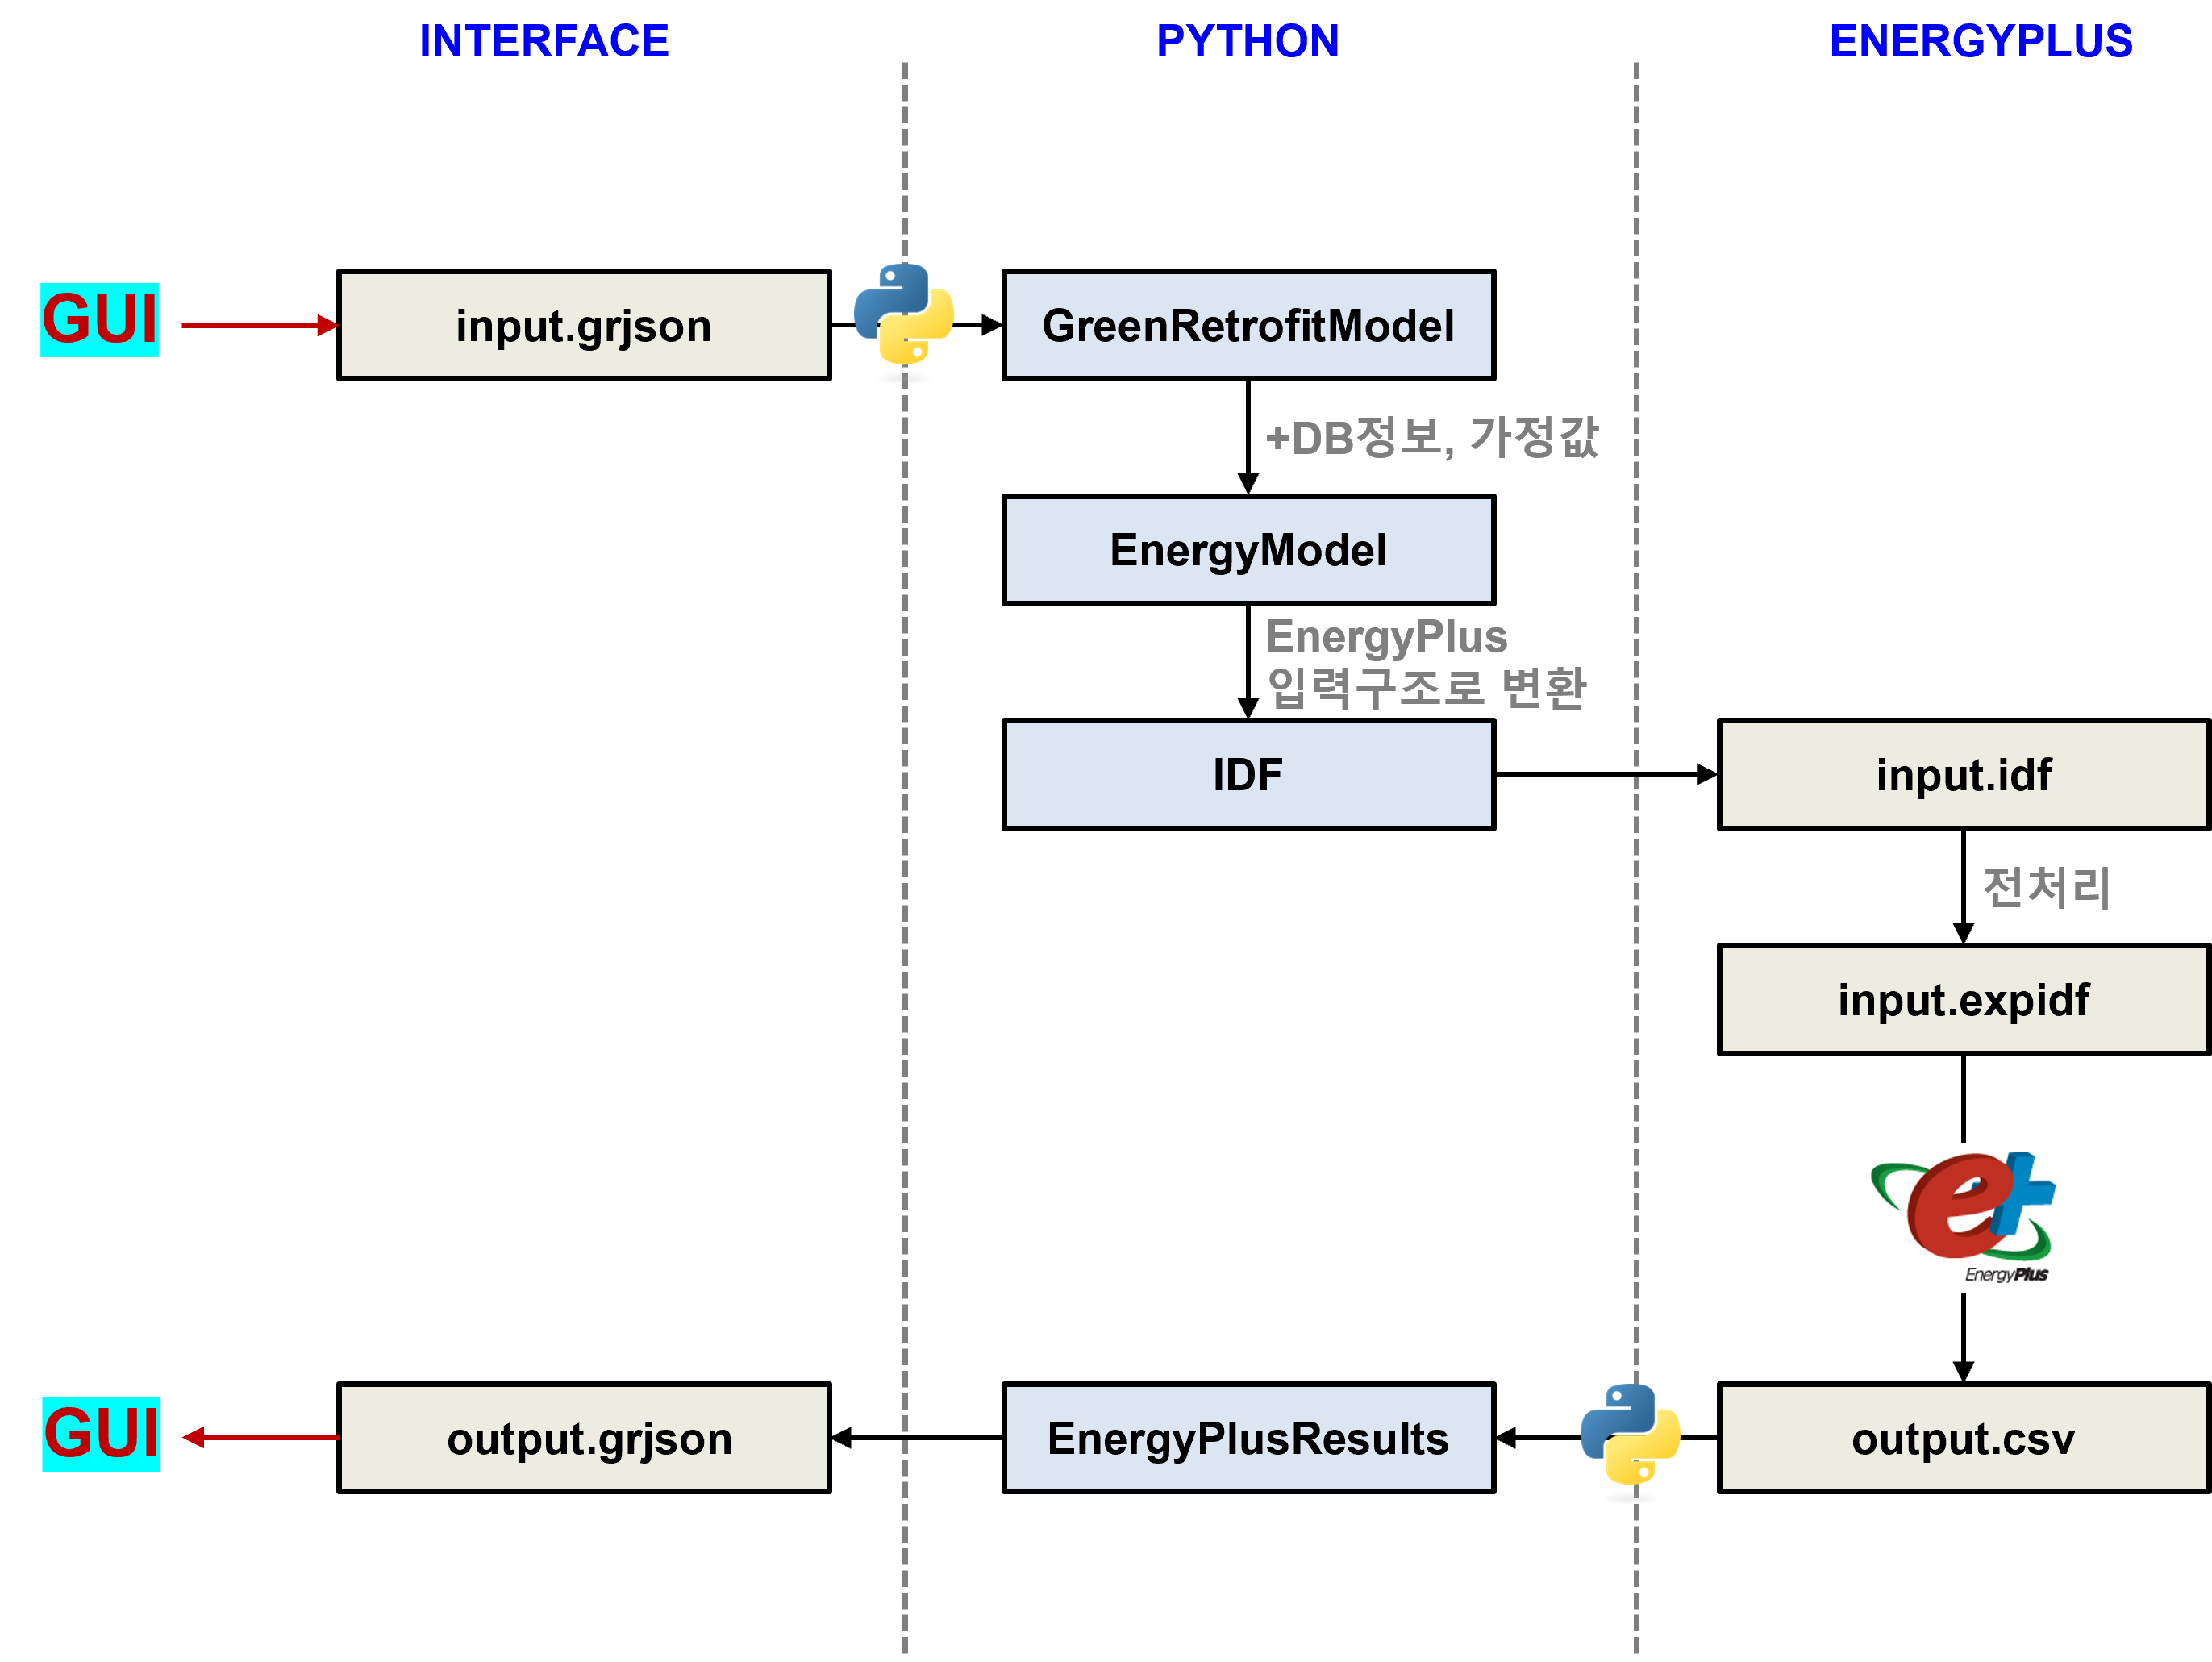
\includegraphics[width=\textwidth]{GRSimulator의 실체.png}
  \caption{\simulator\ 프로그램의 기능...이 무엇인지?}
  \label{fig:package_function}
\end{defaultfigure}
